\chapter{Methodology}

To tackle the issues presented in the previous section, this study will investigate the main aspects behind the development of two hydraulic models with the aim to approximate the behavior of the sanitary sewer network flows continuously in a cold climate influenced by annual snowmelt periods. In the future, the model should be able to cope with existing monitoring infrastructure of \acf{SCADA} and weather forecast data as input to predict the future status of the network. Even though this study does not go as far as description of real implementation of an integrated operational and CSOs/SSOs early warning system, it focuses the development and data acquisition of the hydrological models in real-time operation. It is important to keep in mind the purpose of the model since it influenced decisions of methods to be used and data fetching routines. Thus, key aspects of this study involves:
\begin{itemize}
    \item fetching of real-time monitoring data;
    \item automatic calibration \& validation;
    \item State of network in different nodes;
    \item Transfer times among pumping stations;
    \item 24h forecast: possible overflows, capacities, etc.
\end{itemize}

There is an existent hydraulic model of the study site. Therefore, details about this model are briefly presented later in section \ref{hydraulicmodel}.
Focus is given here to the hydrological model and the methodology was divided in two parts named: 1. Offline Model and 2. Online Model. The first aimed to investigate the model's data necessities, the process of parameter estimation based on spatial data of the study site, and first simulation with previously estimated parameters. The Online Model uses not only historical meteorological events, but also weather forecast for comparing the two proposed hydraulic models results and a preliminary analysis of their performance for real-time applications. 

\section{Offline Model}
First step was the creation of hydrological model and coupling to hydraulic model using \acf{SWMM} developed by the \acf{EPA}. The model was built, calibrated and validated using historical data. The goal of the offline model part was to identify the best set of parameters and how to handle challenging parts such as: initial soil moisture content, soil frost, percentage of rainfall lost to stormwater sewer network, aquifer interations, etc. Figure \ref{fig:offlineflow} shows a simplified flowchart of the hydrological model development steps.


\begin{figure}[h]
    \centering
	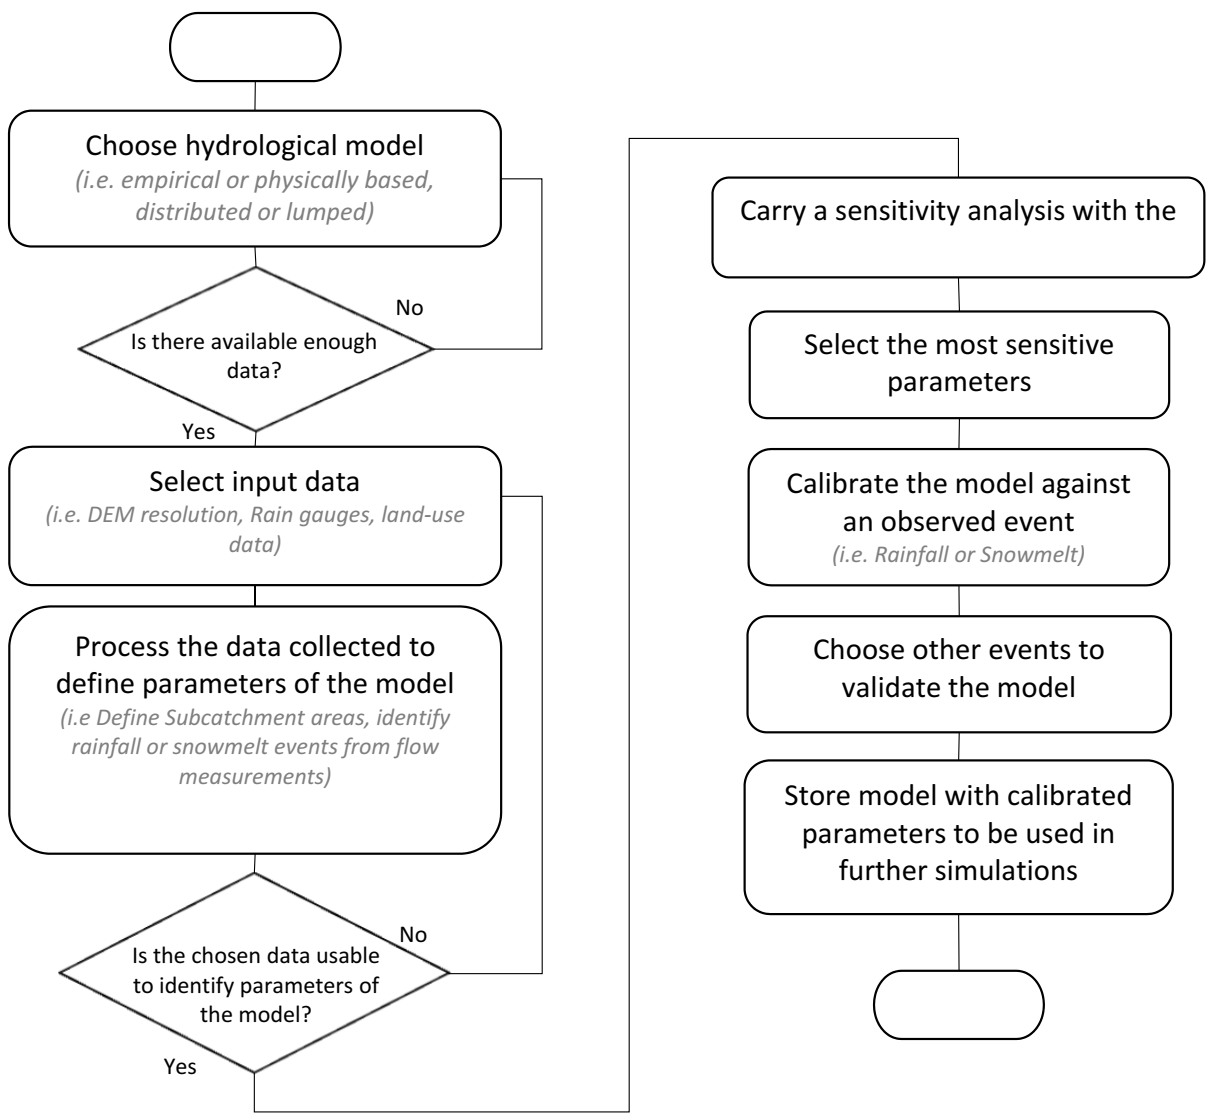
\includegraphics[height=12cm]{figures/Offline_Model_Creation_Flow_Chart.png}
	\caption{Hydrological Model Development Flowchart}
	\label{fig:offlineflow}
\end{figure}



\section{Online Model}

[To Do]

\textbf{This section will aim to answer the questions posed below} \\ \\

This section presents questions related to the continuous simulation process. The answers express initial ideas to explain how the continuous simulation will work and what are the main concerns. 
•	How long will the simulations run? This depends on many factors such as the type of hydrological, hydraulic model, calibration process, routine, hardware used to process the information. 

•	How often will the simulation run? Routine of simulation is constraint by data acquisition routine.  The routine of simulation can also vary during a storm event applying a shorter time of simulation. As an example, imagine if all necessary data to run a simulation is available every 15min and the model takes 30min to run a complete simulation, the iterations necessary for the optimization of parameters during the calibration process can be reduced as an attempt to decrease the time of simulation down to 15min. This could allow a better decision-making process during intense rainfall events, even if some accuracy is compromised.

•	What information is relevant before, during, and after a rainfall or snowmelt event?
Before the rainfall and/or snowmelt: When and where peak flows will happen in the sanitary sewer system. Where and when can CSOs or SSOs can happen. What would be the transfer times between points of the network? During rainfall and/or snowmelt: Status of the system with focus in short-time forecast (+1-2h): Where are the peak flows, CSOs, SSOs, happening and how will then be within 1-2h. Are all the measurement instruments safe and providing good enough data? Maybe a quick check of the input data will be necessary to identify whether the instrument is broken or not. If we cannot rely on the real-time data, what would be the strategy? Maybe use the last reliable data collected to forecast the behavior of the system. After rainfall and/or snowmelt:  Maybe the peak flows will still happen. How long will the flows in the system still be considered RDII and higher than average peak flows of DWF? 

•	Which parameters will be calibrated? According do Choi and Ball (2002) (Choi and Ball 2002) there are two types of parameters related to quantity part of runoff block in SWMM: 1. Measured Parameters; 2. Inferred Parameters. The first are parameters directly measured such length of channels/pipes, catchment land-use, or recorded rainfall depth. The second, parameters not directly measured, and coefficients used by empirical models that approximate complex physical processes. More about this is discussed in section 4.4. Inferred parameters approximate characteristics of the system (i.e. imperviousness) and processes (i.e. flow coefficients such as hydraulic conductivity or manning’s). Inferred parameters are the least known values since no measurements were carried. Therefore, they are the first candidates to be chosen when calibrating since the uncertainties tend to be higher than the measured parameters. A sensitivity analysis will be done during the offline modelling part to identify which of the inferred parameters have greater impact to the results. The inferred parameters with greater impacts will be then chosen for calibration. 

•	Why not all parameters will be calibrated? The number of parameters necessary to run SWMM and the range of possible values for each parameter can be a very large number. This increases the search space for the calibration algorithm where many iterations will be required to identify optimal set of parameters. This can rapidly increase the time of simulation limiting the model’s forecast capability.

•	How will the Automatic Calibration Process work? The automatic calibration will have a routine according to the necessity of the models. A calibration run might happen in scale of hours, days, weeks, months, etc. A new set of parameters will then be proposed and an evaluation to compare whether the new set of parameters is better than the previous one. The frequency of calibration and the possible values of the parameters must be further investigated since less frequent events might have very distinct behavior than more frequent events. It is also possible to define different set of parameters for different seasons and event’s magnitude. An approximated system diagram is shown in figure \ref{fig:diagram}.


\begin{figure}[h]
    \centering
	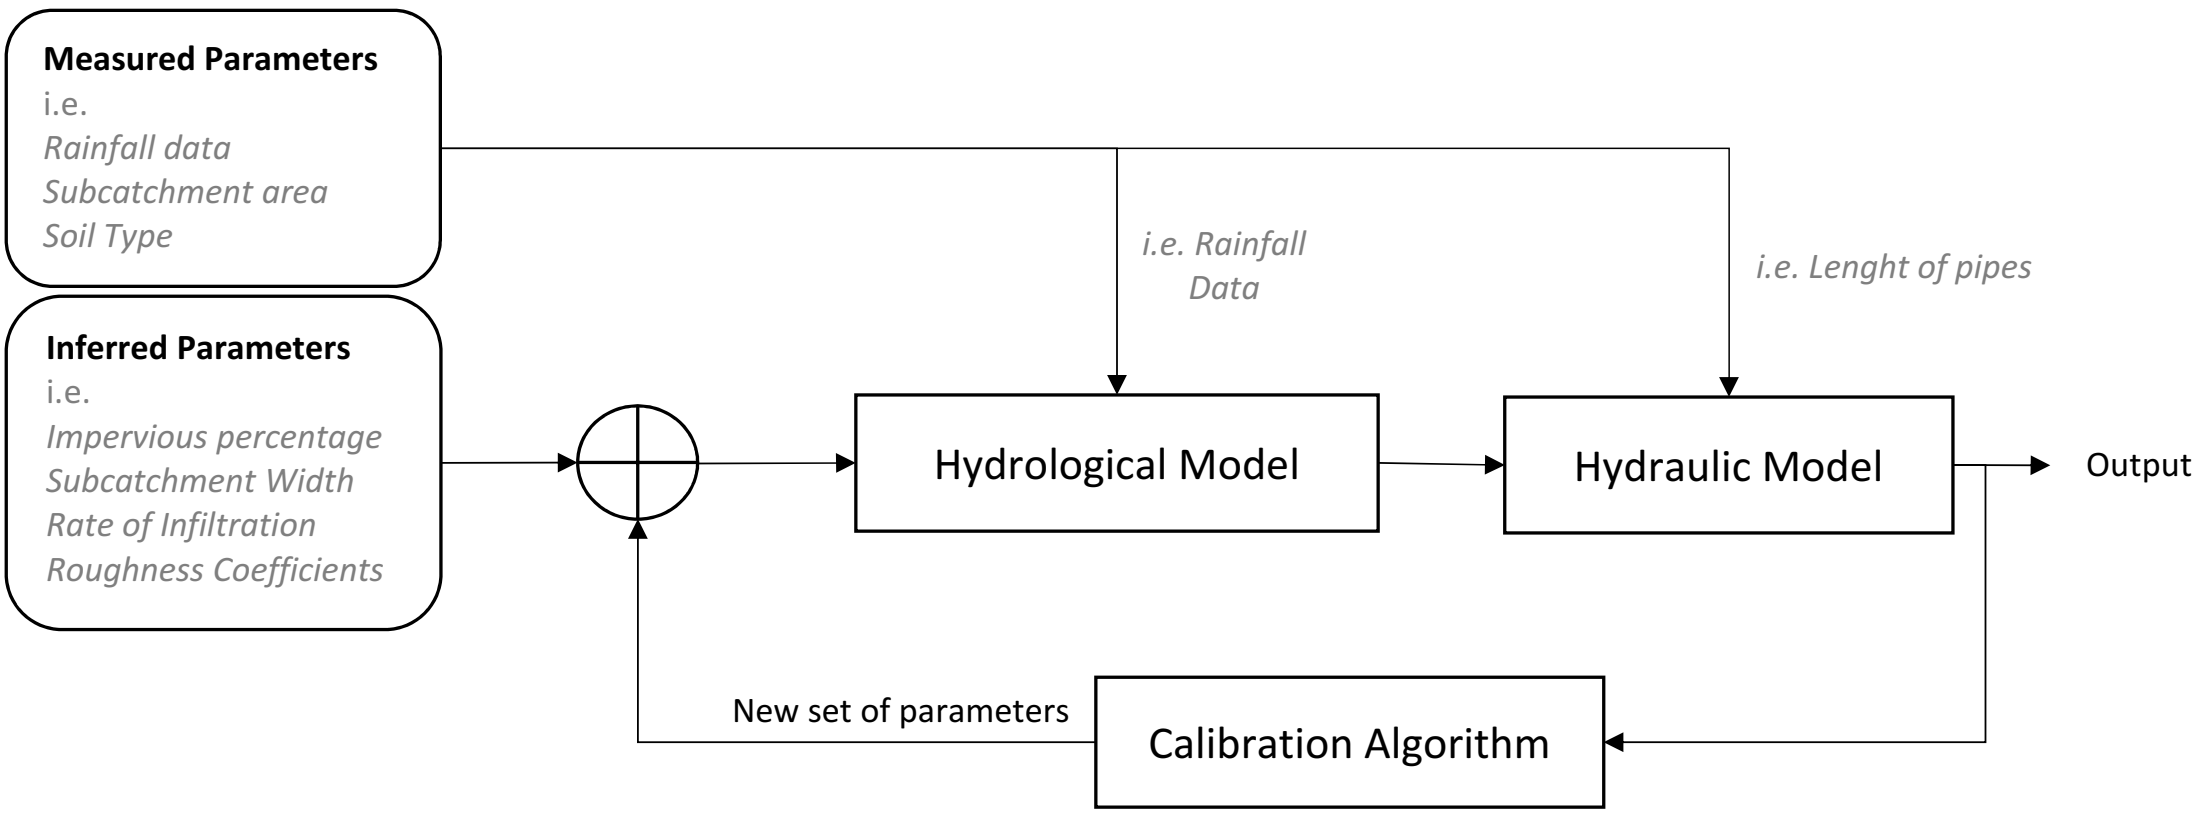
\includegraphics[scale=0.35]{figures/System_Diagram.png}
	\caption{System Diagram}
	\label{fig:diagram}
\end{figure}


\section{Parameter Optimization Algorithm}

\acf{DDS} is a stochastic single-solution based heuristic global search algorithm that was created for the automatic calibration process of watershed simulation models. It was developed to find good global solution for a set of parameters faster than previously available search algorithms. DDS was proposed by \citeauthor{tolson2007} \citeyearpar{tolson2007}  \cite{tolson2007}. 
DDS mimics the process of manual calibration. According to \citet{dent2004} a calibration algorithm workflow can be defined as: 
\begin{enumerate}
    \item Change parameters of the model;
    \item Run the model simulation;
    \item Measure error of simulated vs observed;
    \item Repeat previous steps and choose the most fit set of parameters.
\end{enumerate}
For hydrologic models with multiple subcatchments and parameters, the number of possible combinations of parameters are of several orders of magnitude. This complexity motivates the adoption of optimization algorithms for automatic calibration.   
For a given hydrologic model with only one catchment and three different parameters: area, slope, and roughness. Assuming that area is constant but the other two can assume each five other possible values. The possible combination of parameters to represent the catchment would be 165. Now let’s assume the catchments is divided in two subcatchments. In this case, the possible number of combinations would raise to 74613.
The name Dynamically Dimensioned is given due to the ability of the algorithm to scale the search based on user-specified maximum number of iterations. Global search approach is used for the first iterations. DDS switches to a local search approach by selecting and reducing the search space when the number of iterations nears the maximum allowed. The algorithm reduces the search space by strategic reduction of the number of parameters to be calibrated when it approximates to the end of the search. It also respects the constraints of each parameter given by the user. Therefore, it does not choose values for a parameter out of the specified range.
Other relevant aspects of Automatic Calibration and DDS for SWMM:


\begin{itemize}
    \item Automatic Calibration avoids modelers bias, accelerates the process of calibration, and handles multiple objectives such as peak flows, hydrograph shape, and total volume \cite{dent2004};
    \item DDS was created for computationally expensive calibrations \cite{arsenault2013}. Therefore, it is suitable for SWMM where a possible large number of parameters should be simultaneously optimized;
    \item DDS converges rapidly finding a good solution for a set of parameters and successfully avoid poor local solutions \cite{tolson2007};
    \item For distributed model such as used in SWMM, comparisons available in the literature have proven that DDS is one of the fastest to converge and the best finding good solutions. In other words, DDS does outperform other algorithms for complex models\cite{tolson2007,wallner2012,arsenault2013};
\end{itemize}

\begin{algorithm}
	\caption{Dynamically dimensioned search algorithm by \citet{tolson2007} and algorithm structure presentation by \citet{Sunela2017}}
	\label{alg:dds}
	\begin{algorithmic}
		\State $f_{best} \gets f(\bar{x}_0)$
		\State $\bar{x}_{best} = \bar{x}_0$
		\For {$i \gets 1,\,m$}
		\State \textit{Randomly select the decision variables that will be perturbed.}
		\State $p \gets 1 - \frac{\ln{i}}{\ln{m}}$
		\State $N \gets \emptyset$
		\For {$d \gets 1,\,n$} 	
		\State $X \sim U([0, 1])$
		\State \textbf{if} $X \leq p$ \textbf{then}	$N \gets N \cup \{d\}$
		\EndFor
		\If {$N = \emptyset$}
		\Comment{Ensure variable change}
		\State $X \sim U([1, n])$
		\State $N = \{ X \}$
		\EndIf
		\State \textit{Construct new solution by perturbing the current best}
		\State $\bar{x} \gets \bar{x}_{best}$
		\For {$\forall j \in N$}
		\State $x_j \gets x^{best}_j + r \cdot (x^{max}_j - x^{min}_j) \cdot N([0, 1])$		
		\If{$x_j < x^{min}_j$}
		\State $x_j \gets x^{min}_j + (x^{min}_j - x_j)$
		\State \textbf{if} $x_j > x^{max}_j$ \textbf{then} $x_j \gets x^{min}_j$
		\ElsIf{$x_j > x^{max}_j$}
		\State $x_j \gets x^{max}_j - (x_j - x^{max}_j)$
		\State \textbf{if} $x_j < x^{min}_j$ \textbf{then} $x_j \gets x^{max}_j$
		\EndIf
		\EndFor
		
		\State \textit{Evaluate the objective function value for the new solution}
		\State $f \gets f(\bar{x})$
		\If{$f \leq f_{best}$}
		\State $f_{best} = f$
		\State $\bar{x}_{best} = \bar{x}$
		\EndIf
		\EndFor
	\end{algorithmic}	
\end{algorithm}



 

